\chapter{Design strategies}
We implemented a number of strategies for improving efficiency of raSAT: incremental search and refinement heuristics.
\section{Incremental search} \label{sec:incsearch}
{\bf raSAT} applies three incremental strategies, 
(1) {\em incremental windening}, (2) {\em incremental deepening} and (3) {\em incremental testing}. 
Let
$F = \exists x_1 \in I_1 \cdots x_n \in I_n. \bigwedge \limits_{j=1}^m f_j > 0$
for $I_i = (a_i,b_i)$. %where $a_i, b_i$ would be $\pm \infty$. 

\subsection{Incremental windening}
Given $0 < \delta_0 < \delta_1 < \cdots$, 
{\em incremental windening} starts with 
$F_0 = \exists x_1 \in I_1 \cap (-\delta_0 , \delta_0) \cdots x_n \in I_n \cap (-\delta_0 , \delta_0). 
\bigwedge \limits_{j=1}^m f_j > 0$, 
and if it finishes with UNSAT, it runs with 
$F_1 = \exists x_1 \in I_1 \cap (-\delta_1 , \delta_1) \cdots x_n \in I_n \cap (-\delta_1 , \delta_1). 
\bigwedge \limits_{j=1}^m f_j > 0$, and so on (Fig.~\ref{fig:incwid} (a)). 

Note that if $\delta_i < \infty$, {\bf raSAT} applies an Affine interval; otherwise, 
it uses CI. 
Experiments in Section~\ref{sec:experiment} are performed 
with $\delta_0 = 10$ and $\delta_1 = \infty$.
\begin{figure}[ht]
\begin{minipage}[b]{1.0\linewidth}
\centering
\begin{tabular}{c@{\qquad}c}
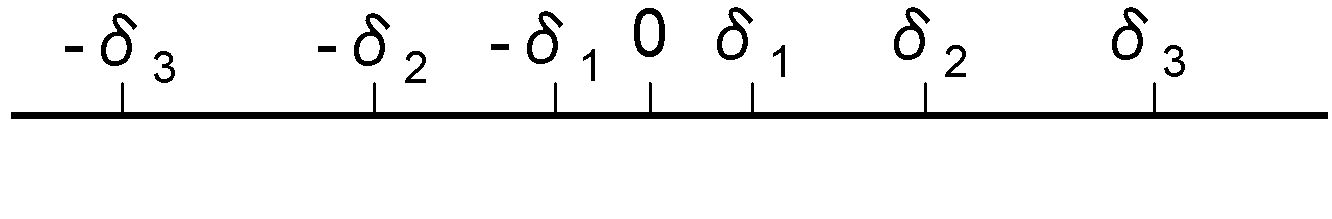
\includegraphics[height=0.4in,width=1.8in]{IncWiden.png} &
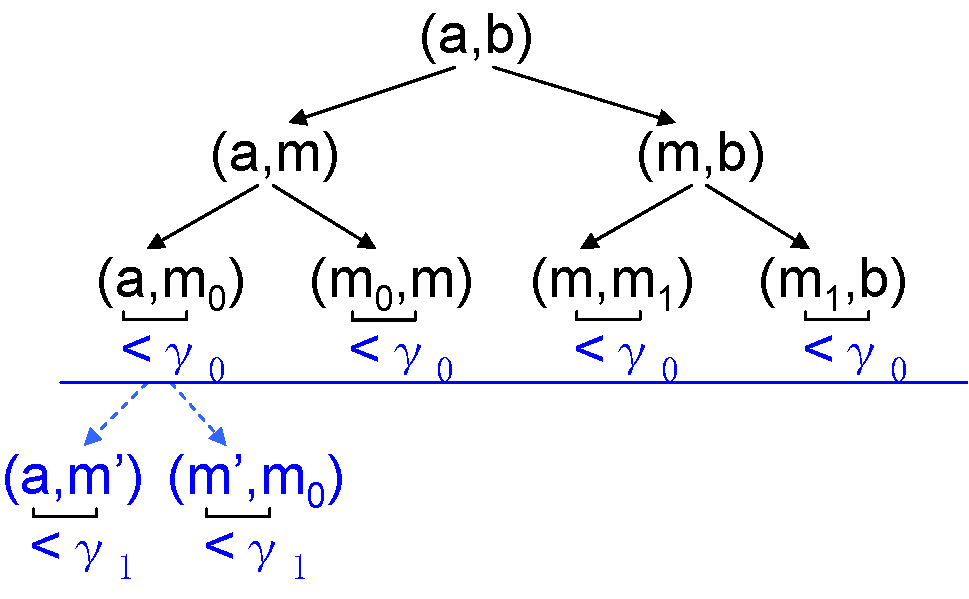
\includegraphics[height=1.2in,width=2in]{IncDeepen.png} \\
\mbox{(a) Incremenal widening} & \mbox{(b) Incremental Deepening} \\
\end{tabular}
\caption{Incremental Widening and Deepening}
\label{fig:incwid}
\end{minipage}
\end{figure}


\subsection{Incremental deepening}

Starting with $F = \exists x_1 \in I_1 \cdots x_n \in I_n. \bigwedge \limits_{j=1}^m f_j > 0$, 
$I_1 \times \cdots \times I_n$ is decomposed into many boxes, 
and $F$ becomes the disjunction of existential formulae corrsponding to these boxes. 
{\bf raSAT} searches these boxes in depth-first manner, which may leads to local optimal search. 
To avoid it, {\bf raSAT} applies a threshold $\gamma$, such that no more decomposition will be 
applied when a box becomes smaller than $\gamma$. 
If neither SAT nor UNSAT is detected, {\bf raSAT} restarts with a smaller threshhold. 

Let $\gamma_0 > \gamma_1 > \cdots > 0$, and {\bf raSAT} incrementally deepens its search 
with these threshholds, i.e., starting with $\delta_0$, and if it fails, restart with $\delta_1$, 
and so on (Fig~\ref{fig:incwid} (b)). 

\section{SAT directed heuristics measure} \label{sec:SATheuristics}

With several hundred variables, we observe that an SMT solver works 
when either SAT, or UNSAT with small UNSAT core.
%
For the latter, we need an efficient heuristics to find an UNSAT core, which is left as future work. 
For the former, the keys are how to choose variables to decompose, and 
how to choose a box to explore. 
{\bf raSAT} chooses such a variable in two steps; first it selects a {\em test-UNSAT API}, and
then chooses a variable that appears in the API. 
We design SAT-directed heuristic measures based on the interval arithemtic ($O.T$). 

Let $F = \exists x_1 \in I_1 \cdots x_n \in I_n. \bigwedge \limits_{j=1}^m f_j > 0$ 
becomes $\vee~( \exists x_1 \in I'_1 \cdots x_n \in I'_n. \bigwedge \limits_{j=1}^m f_j > 0)$ 
after box decomposition. 
For $\exists x_1 \in I'_1 \cdots x_n \in I'_n. \bigwedge \limits_{j=1}^m f_j > 0$, 
if some $f_j > 0$ is UNSAT, the box $I'_1 \times \cdots \times I'_n$ is UNSAT. 
If every $f_j > 0$ is SAT, $F$ is SAT. 
Thus, if the box $I'_1 \times \cdots \times I'_n$ needs to be explore, it must contain 
a test-UNSAT API (thus IA-SAT). 

We denote the estimated range of $f_j$ for $x_1 \in I'_1 \cdots x_n \in I'_n$ with IA ($O.T$)
by $range(f_j, I'_1 \times \cdots \times I'_n)$. 
If an IA is an affine interval, 
it is in the form $[c_1,d_1]\epsilon_1 + \cdots + [c_n,d_n]\epsilon_n$, 
and by instanciating $\epsilon_i$ with $[-1,1]$, 
the resulting classical interval coincides with $range(f_j, I'_1 \times \cdots \times I'_n)$. 
We define 
\begin{itemize} 
\item {\em Sensitivity} of a variable $x_i$ in a test-UNSAT API $f_j > 0$ is $max(|c_i|, |d_i|)$. 
\item {\em SAT-likelyhood} of an API $f_j > 0$ is $| I \cap (0,\infty) | / |I|$, and 
\item {\em SAT-likelyhood} of a box $I'_1 \times \cdots \times I'_n$ is 
the least SAT-likelyhood of test-UNSAT APIs. 
\end{itemize} 

\begin{example} \label{examp:SATlikelyhood}
In Example~\ref{examp:sensitivity}, 
\begin{itemize}
\item sensitivity is estimated $1$ for $x$ and $2$ for $y$ by $AF_2$, and $3\frac{1}{4}$ for $x$ and 
$2$ for $y$. 
\item SAT-likelyhood of $f$ is estimated $0.4= \frac{6}{9-(-6)}$ by $AF_2$ 
and $0.36 = \frac{4.5}{4.5-(-8)}$ by $CAI$. 
\end{itemize}
\end{example}


{\em SAT-likelyhood} intends to estimate APIs how likely to be SAT. 
For choosing variables, {\bf raSAT} first choose a test-UNSAT API by SAT-likelyhood. 
There are two choices, either {\em the largest} or {\em the least}. 
{\em Sensitivity} of a variable intends to estimate how a variable is influencial to the value of an API. 
From a selected API by SAT-likelyhood, {\bf raSAT} selects a variable with the largest sensitivity. 
This selection of variables are used for (1) {\em multiple test instances generation}, and 
(2) {\em decomposition}. 
For test generation, we will select multiple variables by repeating the selection. 

For choosing a box to explore, {\bf raSAT} chooses more likely to be SAT. 
There are two choice, (1) a box with the largest SAT-likelyhood, and 
(2) a box with the largest number of SAT (either IA-valid or test-SAT) APIs. 


\subsection{Over-Approximation Theory Refinement}
\label{sec:soundness}

From now on, We focus on a \emph{polynomial inequality} such that 
$I_i$ and $\psi_j(x_1,\cdots,x_n)$ are an open interval $(a_i,b_i)$ and 
an atomic polynomial inequaltiy (API) $f_j > 0$, respectively. 
We denote $\mathbb{S}(f_j) = \{x \in \Real^n \mid f_j > 0 ~\text{holds}\}$.

For ICP, it is folklore that, for polynomial inequality 
$\exists x_1 \in (a_1,b_1) \cdots x_n \in (a_n,b_n) . \wedge_{i} f_i > 0$, 
\begin{itemize}
\item if $\exists x_1 \in (a_1,b_1) \cdots x_n \in (a_n,b_n) . \wedge_{i} f_i > 0$ is SAT, 
ICP eventually detects it, and 
\item if $\exists x_1 \in [a_1,b_1] \cdots x_n \in [a_n,b_n] . \wedge_{i} f_i \geq 0$ is UNSAT, 
ICP eventually detects it, 
\end{itemize}
under the assumptions of {\em fair} decomposition and bounded intervals $(a_i,b_i)$. 
We will prepare terminology and briefly review this fact. 

%%%%%%%%%%%%%%%%%%%%%%
\suppress{
\begin{definition} \label{def:poly}
A polynomial inequality is a bounded quantification 
$\exists x_1 \in I_1 \cdots x_n \in I_n. \psi(x_1,\cdots,x_n)$ 
such that 
\begin{itemize}
\item each $I_i$ is an open interval $x_i \in (a_i,b_i)$, and 
\item $\psi(x_1,\cdots,x_n)$ is a conjunction of $f_j > 0$ 
where $f_j$ is a polynomial over $\{x_1, \cdots, x_n\}$. 
\end{itemize}
$f_i > 0$ is called an atomic polynomial inequality (API). 
We denote $\mathbb{S}(F) = \{x \in \Real^n \mid F ~\text{holds}\}$.
\end{definition}

\begin{example} \label{examp:poly_ieq}
$\exists x \in (-1,3)~y \in (2,4) . (x^3y - y^4 > 0) \wedge (y^3 -xy >0)$
is an example of a polynomial inequality with 2 variables and 2 APIs. 
\end{example}
}
%%%%%%%%%%%%%%%%%%%%%%

\begin{definition}
An \emph{open box} of dimension $n$ is a set $(a_1,b_1) \times \cdots \times (a_n,b_n)$ 
where $a_i, b_i \in \Real, a_i \leq b_i$.  
For $\mathfrak{a} = (a_1, \cdots, a_n)$ and $\mathfrak{b} = (b_1, \cdots, b_n)$, 
we denote $(a_1,b_1) \times \cdots \times (a_n,b_n)$ by $(\mathfrak{a}, \mathfrak{b})$. 
\end{definition}

The set of all open boxes is a basis of Euclidean topology on $\Real^n$. 
In $\Real^n$, a set $U$ is compact if, and only if, $U$ is a bounded closed set. 
We denote a closure of a set $U$ by $\overline{U}$. 
%
Since a polynomial is continuous, 
$\mathbb{S}(\bigwedge \limits_{i=1}^m f_i > 0)$ is an open set. 
Note that $\Rat$ is dense in $\Real$, and an SAT instance in reals can be replaced with one in rationals. 

%%%%%%%%%%%%%%%%%%%%%%%%%%%%%%
\suppress{
\begin{lemma} \label{cor:rattoreal}
For a polynomial inequality
$F = \exists x_1 \in I_1 \cdots x_n \in I_n. \bigwedge \limits_{j=1}^m f_j > 0$, 
If there exists an SAT instance of F in $\Real^n$, there exists also in $\Rat^n$. 
\end{lemma}

\begin{lemma} \label{cor:refinement}
Suppose that $a_j < b_j$ for $1 \leq j \leq n$ and $f_i$'s are polynomials. 
Assume $a_k < c < b_k$ for some $k$. 
Then, 
$\exists x_1 \in (a_1,b_1) \cdots x_n \in (a_n,b_n). \bigwedge \limits_{i=1}^m f_i > 0$ 
is SAT (resp. UNSAT) if, and only if, 
$\exists x_1 \in (a_1,b_1) \cdots x_k \in (a_k,c) \cdots x_n \in (a_n,b_n). 
 \bigwedge \limits_{i=1}^m f_i > 0 
 \vee 
 \exists x_1 \in (a_1,b_1) \cdots x_k \in (c,b_k) \cdots x_n \in (a_n,b_n)). 
 \bigwedge \limits_{i=1}^m f_i > 0$ 
is SAT (resp. UNSAT). 
\end{lemma}

\begin{pf}
We show for the SAT case. If-part is obvious. For only-if-part, 
since $\mathbb{S}(\bigwedge \limits_{i=1}^m f_i > 0)$ is an open set, 
if $y \in (a_1,b_1) \times \cdots \{c\} \cdots \times (a_n,b_n)$ satisfies 
$\bigwedge \limits_{i=1}^m f_i > 0$, 
there exists $x_1 \in (a_1,b_1) \cdots x_k \in (a_k,c) \cdots x_n \in (a_n,b_n)$
(also $x_1 \in (a_1,b_1) \cdots x_k \in (c,b_k) \cdots x_n \in (a_n,b_n)$) that satisfies
$\bigwedge \limits_{i=1}^m f_i > 0$. 
\end{pf}

Lemma~\ref{cor:rattoreal} says that proving SAT of $F$ in $\Real$ is reduced to 
that in $\Rat$. 
Lemma~\ref{cor:refinement} says that, in the refinement step, we can apply refinement 
$x_k \in (a_k,b_k)$ to $x_k \in (a_k,c) \vee x_k \in (c,b_k)$, 
instead of $x_k \in (a_k,c] \vee x_k \in (c,b_k) $
(i.e., $c$ is ignored). 
}
%%%%%%%%%%%%%%%%%%%%%%%%%%%%%%

Initially, interval constraints consists of conjunction only. Later, by refinements, it becomes a CNF. 


%\begin{example} \label{examp:poly_ieq}
$\exists x \in (-1,3)~y \in (2,4) . (x^3y - y^4 > 0) \wedge (y^3 -xy >0)$
is an example of a polynomial inequality with 2 variables and 2 APIs. 

For instance, $x \in (-1,3)$ and $y \in (2,4)$ are refined to smaller intervals
such that 
$\exists x \in (-1,1) y \in (2,4) . (x^3y - y^4 > 0) \wedge (y^3 -xy >0) \vee 
 \exists x \in (1,3) y \in (2,4) . (x^3y - y^4 > 0) \wedge (y^3 -xy >0)$, 
which results a CNF 
$(x \in (-1,1) \vee x \in (1,3)) \wedge (y \in (2,4)) \wedge (x^3y - y^4 > 0) \wedge (y^3 -xy >0)$.
%(only the CNF formula $(x \in (-1,1) \vee x \in (1,3)) \wedge (y \in (2,4))$ is given to SAT solver).
%\mizuhito{could you fulfill? Direct encoding seems a DNF?}. 
%\end{example}

Note that an interval arithmetic used in ICP is a converging theory. 

\begin{definition} \label{def:completeOT}
Let
$F = \exists x_1 \in I_1 \cdots x_n \in I_n. \bigwedge \limits_{j=1}^m f_j > 0$
be a polynomial inequality such that each $I_i$ is bounded. 
An over-approximation theory $O.T$ is {\em converging} 
if, for each $\delta > 0$ and $c = (c_1, \cdots, c_n) \in I_1 \times \cdots \times I_n$, 
there exists $\gamma > 0$ such that 
$\bigwedge \limits_{j=1}^n x_j \in (c_j - \gamma, c_j + \gamma) \models_{O.T} 
 \bigwedge \limits_{i=1}^m (f_i(c) - \delta < f_i(x) < f_i(c) + \delta)$. 
\end{definition}

$O.T$ refinemnet loop is shown in Fig.~\ref{fig:OTrefine}~(a). 
A standard ICP based algorithm of an SMT solver applies it with $O.T$ as a classical interval arithemtic. 
The variation of interval arithemtic will be presented in Section~\ref{sec:approximation}. 
\begin{figure}[ht]
\begin{minipage}[b]{1.0\linewidth}
\centering
\begin{tabular}{c@{\qquad}c}
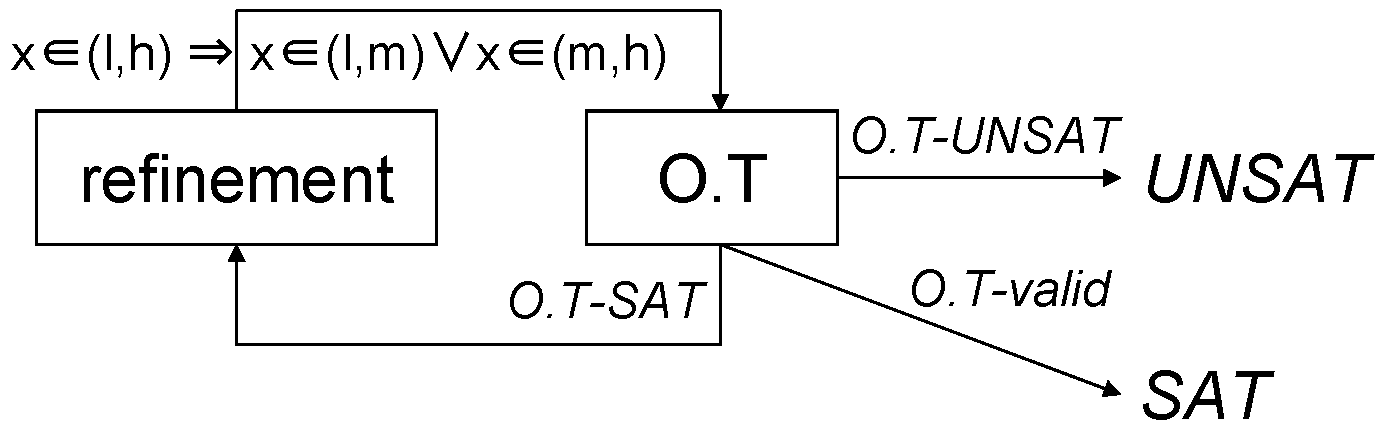
\includegraphics[height=0.6in,width=1.7in]{OTloop.png} & 
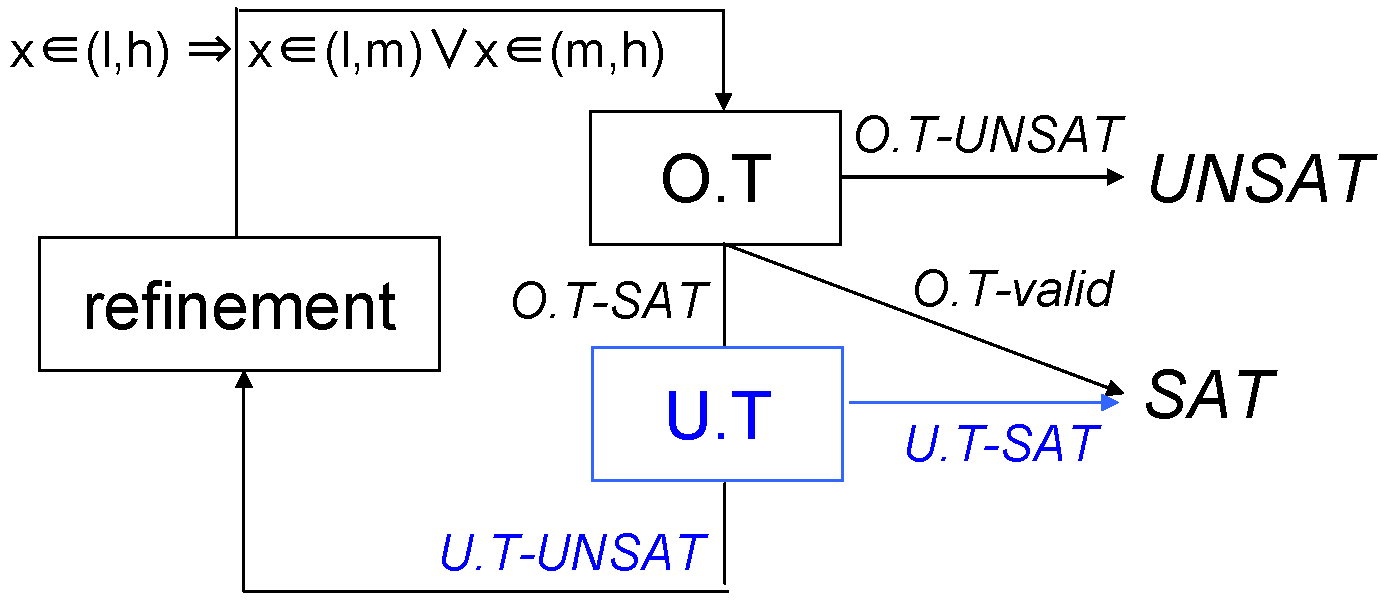
\includegraphics[height=0.9in,width=1.7in]{rasatloop.png} \\   
\mbox{(a) $O.T$ refinement loop} & \mbox{{\bf raSAT} loop} \\
\end{tabular}
\end{minipage} 
\caption{Rfinement loops} 
\label{fig:OTrefine} 
\end{figure}


\begin{definition} 
Let
$F = \exists x_1 \in I_1 \cdots x_n \in I_n. \bigwedge \limits_{j=1}^m f_j > 0$
for $I_i = (a_i,b_i)$.
A refinement strategy is {\em fair}, if, for each $c_j \in (a_j,b_j)$ and $\gamma > 0$, 
a decomposition of $I_i$ for each $i$ eventually occurs in $(c_j - \gamma, c_j + \gamma)$ 
(as long as neither SAT nor UNSAT is detected). 
\end{definition}

\begin{theorem} \label{th:RelComp}
Let
$F = \exists x_1 \in I_1 \cdots x_n \in I_n. \bigwedge \limits_{j=1}^m f_j > 0$
for $I_i = (a_i,b_i)$.
Assume that an over-approximation theory $O.T$ is converging, 
each $(a_i,b_i)$ is bounded, and a refinement strategy is fair. 
Then, 
\begin{itemize}
\item if $\exists x_1 \in (a_1,b_1) \cdots x_n \in (a_n,b_n) . \wedge_{i} f_i > 0$ is SAT, 
$O.T$ refinemnet loop eventually detects it, and
\item if $\exists x_1 \in [a_1,b_1] \cdots x_n \in [a_n,b_n] . \wedge_{i} f_i \geq 0$ is UNSAT, 
$O.T$ refinement loop eventually detects it.  
\end{itemize}
\end{theorem}


\begin{proof} 
The former is proved by the fact that, if $F$ is SAT, there exists a non-empty neiborhood (open box) 
in $\cap~\mathbb{S}(f_j)$. 
If the box decomposition strategy is fair, the refinemnet will eventually find such an open box. 

For the latter, assume that 
$\overline{F} = \exists x_1 \in [a_1,b_1] \cdots x_n \in [a_n,b_n] . \wedge_{i} f_i \geq 0$ is UNSAT. 
Thus, $\cap~\overline{\mathbb{S}(f_i)} = \emptyset$. 
Let $\delta_{j,k} = min \{|f_j(\bar{x}) - f_k(\bar{x})| \mid \bar{x} \in I_1 \times \cdots \times I_n\}$. 
Since $f_i$'s are continuous and $\overline{I_i}$'s are compact, $\delta_{j,k}$ is well defined,
and $\delta_{j.k} > 0$ for some $j,k$. 
Let $\delta = \frac{min \{ \delta_{j,k} \}}{2}$. 
Since $O.T$ is converging, there exists $\gamma > 0$ for $\delta > 0$ 
satisfying Definition~\ref{def:completeOT}, and fair decomposition eventually finds open boxes
such that $\mathbb{S}(f_j)$ and $\mathbb{S}(f_k)$ are separated. 
%\qed
\end{proof}

Limitations for detecting UNSAT occur on \emph{kissing} and \emph{convergent} cases. 
Fig.~\ref{fig:limit} left shows a kissing case 
$x^2 + y^2 < 2^2 \wedge (x-4)^2 + (y-3)^2 < 3^2$ such that 
$\overline{\mathbb{S}(- x^2 - y^2 + 2^2)} \cap \overline{\mathbb{S}(- (x-4)^2 - (y-3)^2 + 3^2)} 
= \{(x,y) \mid (1.6, 1.2)\}$. 
Thus, there are no coverings to separate them. 
%$x^2 + y^2 < 2^2$ and $(x-4)^2 + (y-3)^2 < 3^2$. 
%
Fig. \ref{fig:limit} right shows a convergent case 
$y > x + \frac{1}{x} \wedge y < x \wedge x > 0$, which is equivalent to 
$xy > x^2 + x \wedge y < x \wedge x > 0$. 
%The open box is $(0,\infty) \times (0,\infty)$ and 
There are no finite coverings to separate them. 
%$y > x + \frac{1}{x}$ and $y < x$ for $x > 0$. 

\begin{figure}[ht]
%\begin{minipage}[b]{1.0\linewidth}
\centering
\begin{tabular}{cc}
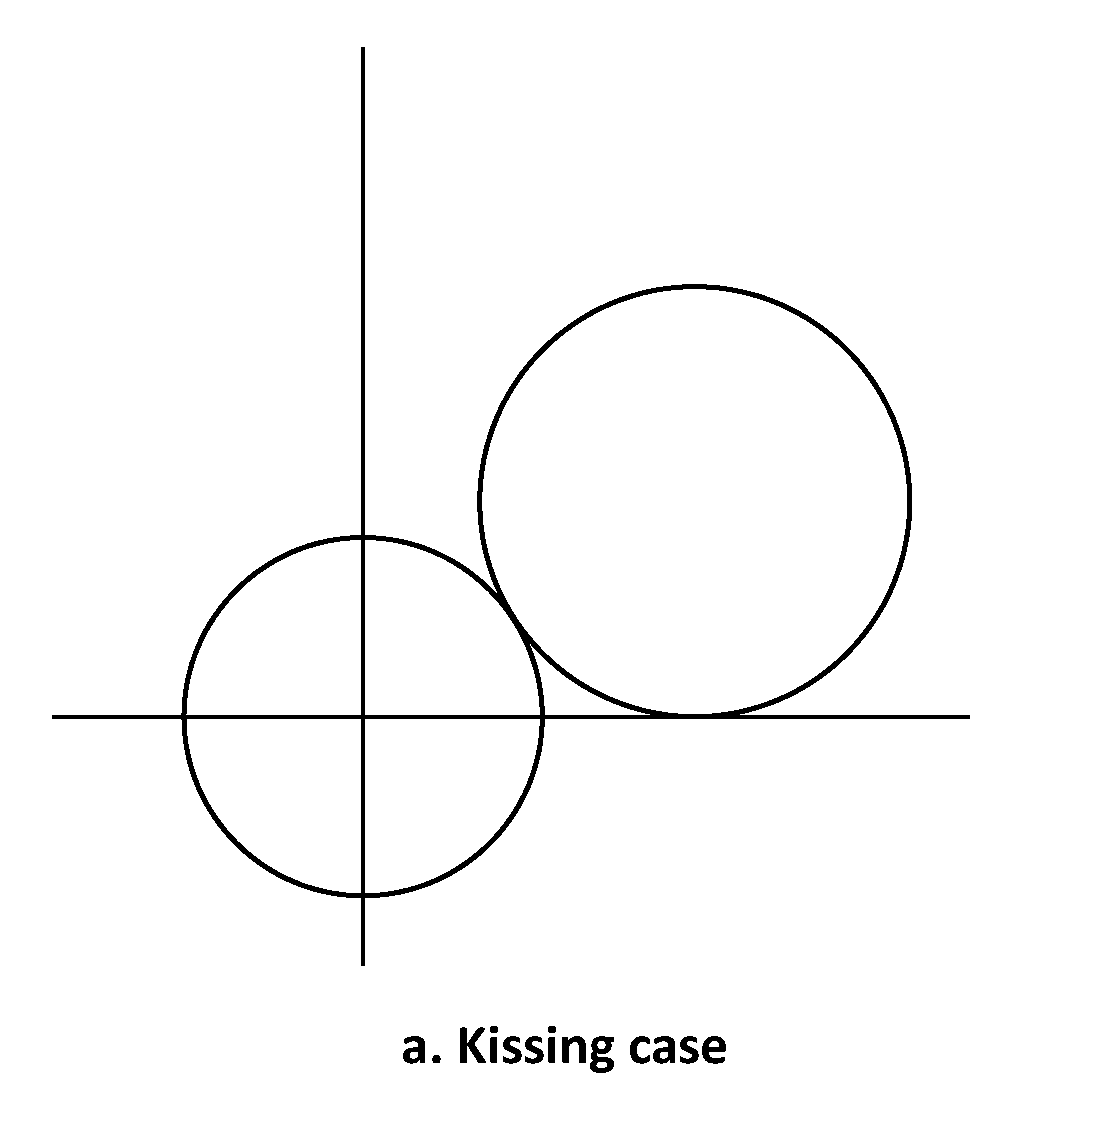
\includegraphics[height=1.65in,width=1.7in]{kissing.eps} &
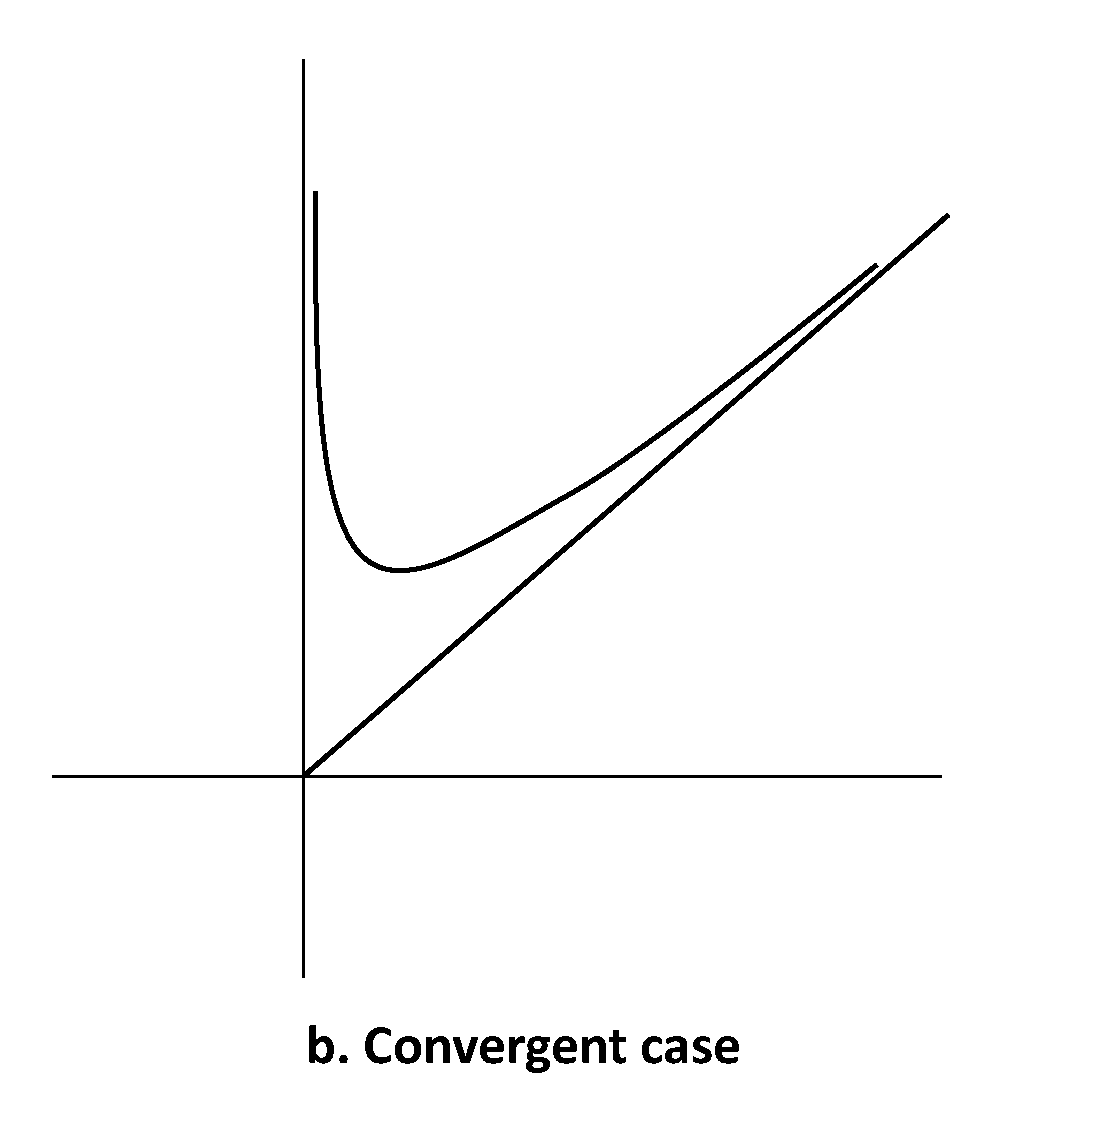
\includegraphics[height=1.65in,width=1.7in]{convergence.eps}
\end{tabular}
\caption{Limitations for proving UNSAT} 
\label{fig:limit} 
%\end{minipage}
\end{figure} 